\documentclass[aspectratio=169,handout]{beamer}
% \usepackage[utf8]{inputenc}
\usetheme{metropolis}
\usecolortheme{orchid}
\usepackage{amsmath}
\usepackage{amssymb}
\usepackage{amsthm}
\usepackage{multirow}
\usepackage[ruled]{algorithm2e}
\usepackage{mathtools}
\usepackage{caption}
\usepackage{epstopdf}
\usepackage{hyperref}
\setbeamerfont{footnote}{size=\tiny}

\usepackage{tikz}
\usetikzlibrary{mindmap,shadows,tikzmark,positioning,arrows.meta}

% Information boxes
\newcommand*{\info}[4][16.3]{%
  \node [ annotation, #3, scale=0.65, text width = #1em,
          inner sep = 2mm ] at (#2) {%
  \list{$\bullet$}{\topsep=0pt\itemsep=0pt\parsep=0pt
    \parskip=0pt\labelwidth=8pt\leftmargin=8pt
    \itemindent=0pt\labelsep=2pt}%
    #4
  \endlist
  };
}

\tikzset{%
  >={Latex[width=2mm,length=2mm]},
  % Specifications for style of nodes:
            base/.style = {rectangle, rounded corners, draw=black,
                           minimum width=4cm, minimum height=1cm,
                           text centered, font=\sffamily},
  activityStarts/.style = {base, fill=blue!30},
       startstop/.style = {base, fill=red!30},
    activityRuns/.style = {base, fill=green!30},
         process/.style = {base, minimum width=2.5cm, fill=orange!15,
                           font=\ttfamily},
}
\renewcommand\textbullet{\ensuremath{\bullet}}
\newcommand\scalemath[2]{\scalebox{#1}{\mbox{\ensuremath{\displaystyle #2}}}}
\newcommand{\norm}[1]{\left\lVert#1\right\rVert}

%%% Bibliography
\usepackage[citestyle=numeric,style=numeric,backend=biber,doi=false,isbn=false,url=false]{biblatex}
\addbibresource{references.bib}

%%% Suppress biblatex annoying warning
\usepackage{silence}
\WarningFilter{biblatex}{Patching footnotes failed}

%%% new theorems %%%%%%%%%%%%%%%%%%%%%%%%%%%%%%%%%%%%%%%%%%%%%%%%%%%%%%%%%%%%%%
\theoremstyle{definition}
\newtheorem{mydef}{Definition}

\theoremstyle{plain}
\newtheorem{mylemma}{Lemma}[section]
\newtheorem{mytheorem}{Theorem}[section]
\newtheorem{myproposition}{Proposition}[section]
\newtheorem{myproblem}{Problem}[section]
\newtheorem{mydefinition}{Definition}[section]
\newtheorem{myassumption}{Assumption}[section]

\theoremstyle{remark}
\newtheorem{myremark}{Remark}[section]

\newcounter{saveenumi}
\newcommand{\seti}{\setcounter{saveenumi}{\value{enumi}}}
\newcommand{\conti}{\setcounter{enumi}{\value{saveenumi}}}

\resetcounteronoverlays{saveenumi}

\title{Controles}
\subtitle{\small Clase 2: Modelos de Sistemas - Tipos de Respuesta - Parámetros de Desempeño}
\author{Gerardo Becerra, Ph.D.}
\institute{Pontificia Universidad Javeriana\\ Departamento de Electrónica}
\date{Enero 29, 2020}

\begin{document}

\frame{\titlepage}	

% \frame{\tableofcontents}

\section{Modelos Matemáticos de Sistemas Dinámicos}
\begin{frame}[<+->]\frametitle{Modelos Matemáticos de Sistemas Dinámicos}
\begin{itemize}
  \item Para entender y controlar sistemas se requiere obtener modelos cuantitativos.
  \item Modelos $\rightarrow$ análisis de relaciones entre variables del sistema.
  \item Sistemas dinámicos $\rightarrow$ representados por ecuaciones diferenciales.
  \item Ecuaciones diferenciales lineales $\rightarrow$ usando la transformada de Laplace se pueden obtener funciones de transferencia.
  \item Linealización $\rightarrow$ herramienta para obtener modelos de sistemas físicos.
\end{itemize}
\end{frame}

\begin{frame}[<+->]\frametitle{Procedimiento para Modelamiento de Sistemas}
\begin{enumerate}
  \item Definir el sistema y sus componentes.
  \item Formular las relaciones básicas entre variables y suposiciones usando los principios fundamentales.
  \item Obtener las ecuaciones diferenciales que representan el modelo matemático.
  \item Solucionar las ecuaciones para las variables deseadas.
  \item Examinar las soluciones y las suposiciones.
  \item En caso necesario, analizar o diseñar el modelo nuevamente.
\end{enumerate}
\end{frame}

\begin{frame}[<+->]\frametitle{Ecuaciones Diferenciales de Sistemas Físicos - Variables y Parámetros}
  \begin{itemize}
    \item Variables pasantes: $F$ (fuerza), $T$ (torque), $i$ (corriente), $Q$ (flujo volumétrico), $q$ (flujo de calor).
    \item Variables transversales: $v$ (velocidad traslacional), $\omega$ (velocidad angular), $V$ (voltaje), $P$ (presión), $\mathcal{T}$ (temperatura).
    \item Almacenamiento inductivo: $L$ (inductancia), $1/k$ (rigidez traslacional o rotacional inversa), $I$ (inertancia).
    \item Almacenamiento capacitivo: $C$ (capacitancia), $M$ (masa), $J$ (momento de inercia), $C_f$ (capacitancia de fluido), $C_t$ (capacitancia térmica).
    \item Disipación de energía: $R$ (resistencia), $b$ (fricción viscosa), $R_f$ (resistencia de fluido), $R_f$ (resistencia térmica).
  \end{itemize}
\end{frame}

\begin{frame}[<+->]\frametitle{Ecuaciones Diferenciales de Sistemas Físicos - Relaciones Fundamentales}
\centering
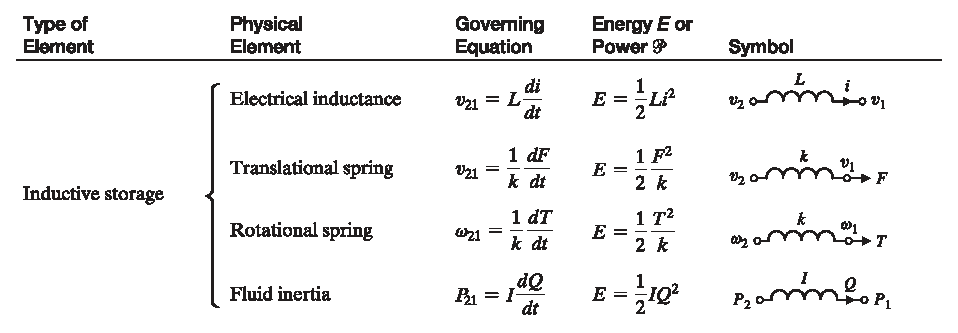
\includegraphics[width=14cm]{images/inductance.eps}
\end{frame}

\begin{frame}[<+->]\frametitle{Ecuaciones Diferenciales de Sistemas Físicos - Relaciones Fundamentales}
\centering
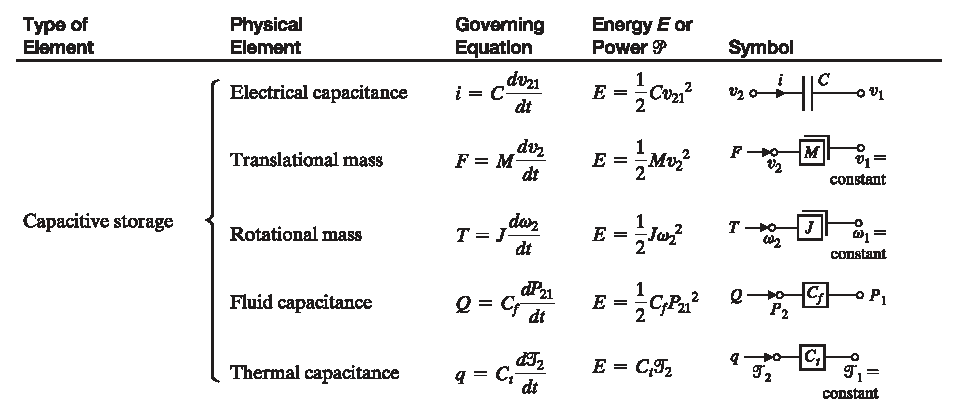
\includegraphics[width=14cm]{images/capacitance.eps}
\end{frame}

\begin{frame}[<+->]\frametitle{Ecuaciones Diferenciales de Sistemas Físicos - Relaciones Fundamentales}
\centering
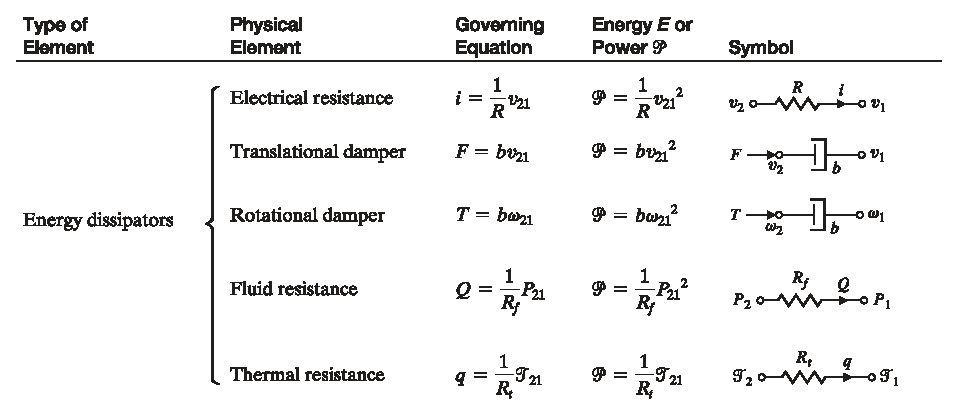
\includegraphics[width=14cm]{images/disipation.eps}
\end{frame}

\begin{frame}[<+->]\frametitle{Modelos de Sistemas - Ejemplo 1}
\centering
\includegraphics[width=9cm]{images/circuit1.eps}
\begin{itemize}
  \item Obtener las ecuaciones diferenciales que describen el sistema.
  \item Obtener la representación en variables de estado.
  \item Obtener la función de transferencia.
\end{itemize}
\end{frame}

\begin{frame}[<+->]\frametitle{Modelos de Sistemas - Ejemplo 1}
\textbf{Ecuaciones diferenciales:}
\begin{subequations}\label{eq:diff_eqs}
\begin{align}
  \frac{di_{L_1}(t)}{dt} &= -\frac{R_1}{L_1}i_{L_1}(t) - \frac{1}{L_1} v_c(t) + \frac{1}{L_1} v_i(t) \\
  \frac{di_{L_2}(t)}{dt} &= -\frac{R_2}{L_2}i_{L_2}(t) + \frac{1}{L_2} v_c(t) \\
  \frac{dv_c(t)}{dt} &= \frac{1}{C}i_{L_1}(t) - \frac{1}{C}i_{L_2}(t)
\end{align}
\textbf{Ecuación de salida:}
\begin{equation}
  V_o(t) = R_2 i_{L_2}(t)
\end{equation}
\end{subequations}
\end{frame}

\begin{frame}[<+->]\frametitle{Modelos de Sistemas - Ejemplo 1}
\textbf{Diagrama de bloques y respuesta paso:}\\
\vspace*{3mm}
\centering
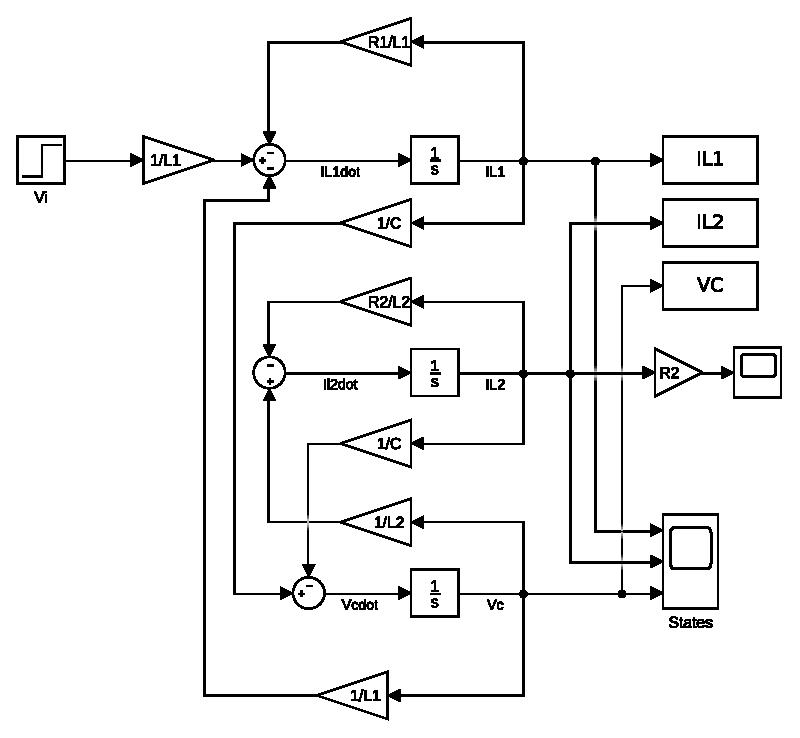
\includegraphics[width=6.5cm]{code/example1_blockdiagram.eps}
\pause
\hspace*{5mm}
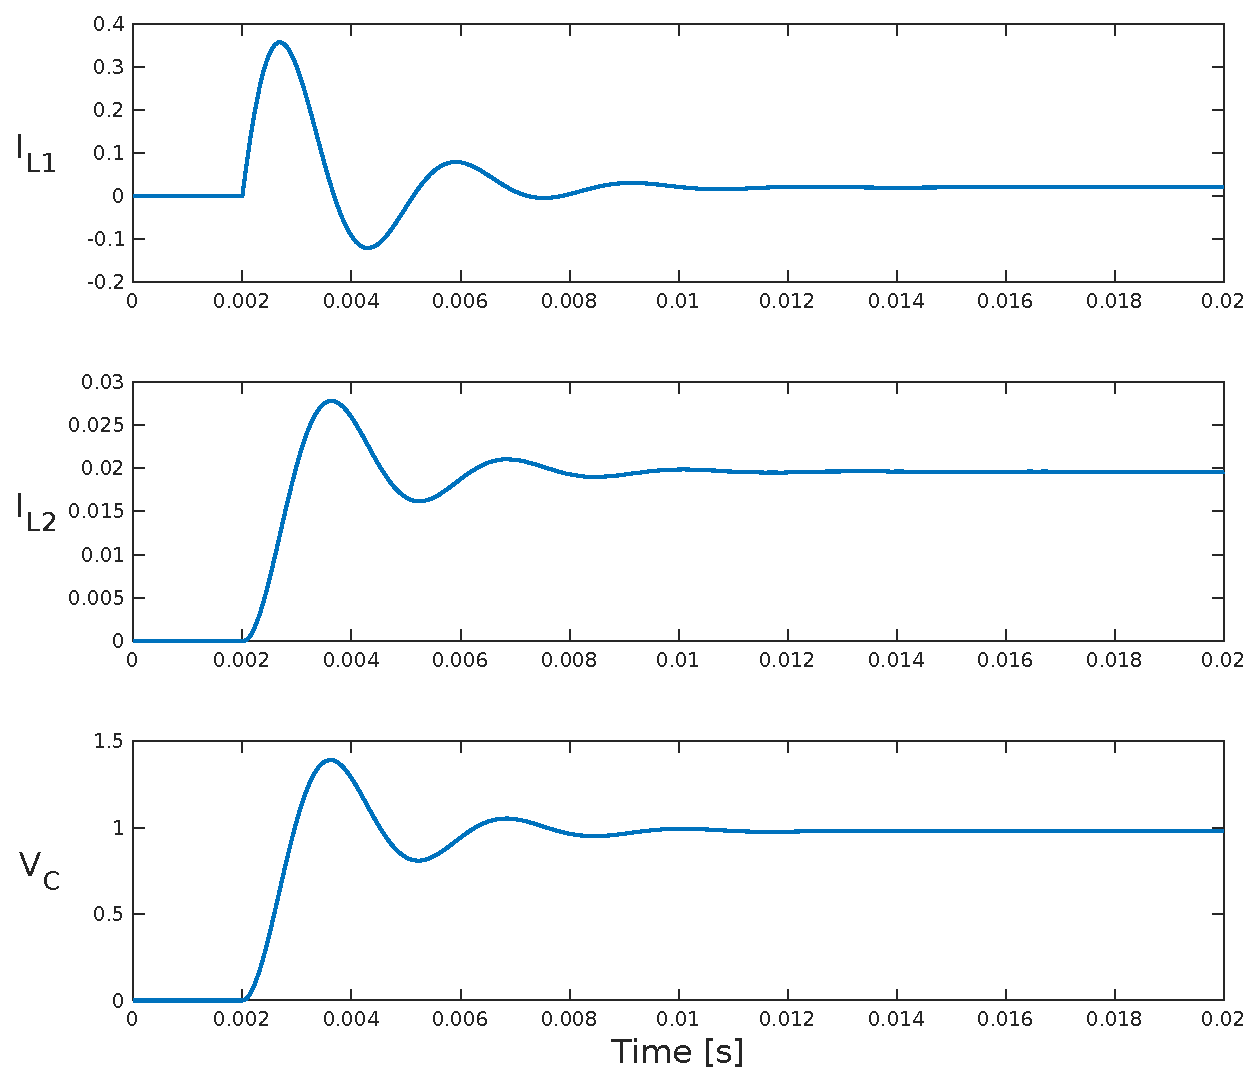
\includegraphics[width=6.5cm]{code/example1_stepresponse.eps}
\end{frame}

\begin{frame}[<+->]\frametitle{Modelos de Sistemas - Ejemplo 1}
Organizando las ecs. \eqref{eq:diff_eqs} en forma matricial:
\begin{subequations}
\begin{align}
  \begin{bmatrix}
   \frac{di_{L_1}(t)}{dt} \\ \frac{di_{L_2}(t)}{dt} \\ \frac{dv_c(t)}{dt} 
  \end{bmatrix} &= 
  \begin{bmatrix}
  -\frac{R_1}{L_1} & 0 & -\frac{1}{L_1} \\
  0 & -\frac{R_2}{L_2} &  \frac{1}{L_2} \\
  \frac{1}{C} & -\frac{1}{C} & 0
  \end{bmatrix}
  \begin{bmatrix}
   i_{L_1}(t) \\ i_{L_2}(t) \\ v_c(t) 
  \end{bmatrix} + 
  \begin{bmatrix}
    \frac{1}{L_1} \\ 0 \\ 0
  \end{bmatrix} v_i(t)\\
  v_o(t) &=
  \begin{bmatrix}
    0 & R_2 & 0
  \end{bmatrix}
  \begin{bmatrix}
   i_{L_1}(t) \\ i_{L_2}(t) \\ v_c(t) 
  \end{bmatrix} + 
  \begin{bmatrix}
    0
  \end{bmatrix} v_i(t)
\end{align}
\end{subequations}
se obtiene la representación en variables de estado:
\begin{subequations}
  \begin{align}
    \dot{x}(t) &= \mathbf{A} x(t) + \mathbf{B}u(t)\\
    y(t) &= \mathbf{C}x(t) + \mathbf{D}u(t)
  \end{align}
\end{subequations}
\end{frame}

\begin{frame}[<+->]\frametitle{Modelos de Sistemas - Ejemplo 1}
Aplicando la transformada de Laplace a las Ecs. \eqref{eq:diff_eqs}:
\begin{subequations}\label{eq:algebraic_eqs}
\begin{align}
  s I_{L_1}(s) &= -\frac{R_1}{L_1}I_{L_1}(s) - \frac{1}{L_1} V_c(s) + \frac{1}{L_1} V_i(s) \\
  s i_{L_2}(s) &= -\frac{R_2}{L_2}I_{L_2}(s) + \frac{1}{L_2} V_c(s) \\
  s V_c(s) &= \frac{1}{C}I_{L_1}(s) - \frac{1}{C}I_{L_2}(s)\\
  V_o(s) &= R_2 I_{L_2}(s)
\end{align}
\end{subequations}
\vspace*{-5mm}
\begin{itemize}
  \item \textbf{Objetivo:} A partir de las Ecs. \eqref{eq:algebraic_eqs}, obtener $V_o(s)/V_i(s)$.
  \item \textbf{Procedimiento:} Manipulación Algebráica.
  \item \textbf{Alternativa:} Usando la representación en variables de estado.
\end{itemize}
\end{frame}

\begin{frame}[<-+>]\frametitle{Modelos de Sistemas - Ejemplo 1}
  Usando la fórmula:
  \begin{equation}
    H(s) = \mathbf{C}(s\mathbf{I}-\mathbf{A})^{-1}\mathbf{B} + \mathbf{D}
  \end{equation}
  se obtiene la función de transferencia:
  \begin{equation}
    H(s) = \frac{2\times10^{11}}{s^3 + 5.1\times10^4 s^2 + 5.6\times10^7 s + 2.02\times10^{11}}
  \end{equation}
\end{frame}

\section{Tipos de Respuesta Transitoria}
\begin{frame}[<-+>]\frametitle{Tipos de Sistemas}
\begin{itemize}
  \item Sistemas de \textbf{primer orden}:
  \begin{equation*}
    H(s) = \frac{K}{\tau s + 1}
  \end{equation*}
  \item Sistemas de \textbf{primer orden con tiempo muerto}:
  \begin{equation*}
    H(s) = \frac{K e^{-Ls}}{\tau s + 1}
  \end{equation*}
  \item Sistemas de \textbf{segundo orden}:
  \begin{equation*}
    H(s) = \frac{\omega_n^2}{s^2 + 2 \zeta \omega_n s + \omega_n^2}
  \end{equation*}
\end{itemize}
\end{frame}

\begin{frame}[<-+>][c]\frametitle{Sistemas de Primer Orden - Respuesta Paso}
\vspace*{3mm}
\begin{columns}
 \begin{column}{0.3\textwidth}
  \begin{equation*}
    H(s) = \frac{K}{\tau s + 1}
  \end{equation*}
  $K$: Ganancia\\
  $\tau$: Constante de tiempo
 \end{column} 
 \begin{column}{0.7\textwidth}
  \centering
  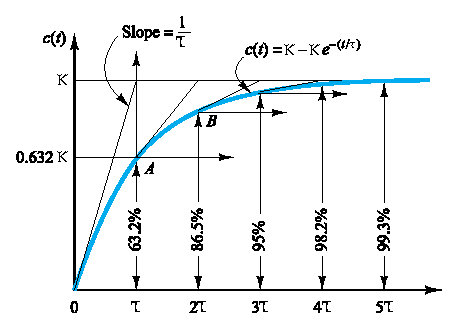
\includegraphics[width=10cm]{images/firstOrderResponse.eps}
 \end{column} 
\end{columns}
\end{frame}

\begin{frame}[<-+>]\frametitle{Sistemas de Primer Orden mas Tiempo Muerto - Respuesta Paso}
\vspace*{3mm}
\begin{columns}
 \begin{column}{0.3\textwidth}
  \begin{equation*}
    H(s) = \frac{K e^{-Ls}}{\tau s + 1}
  \end{equation*}
  $K$: Ganancia\\
  $\tau$: Constante de tiempo\\
  $L$: Tiempo muerto
 \end{column} 
 \begin{column}{0.7\textwidth}
  \centering
  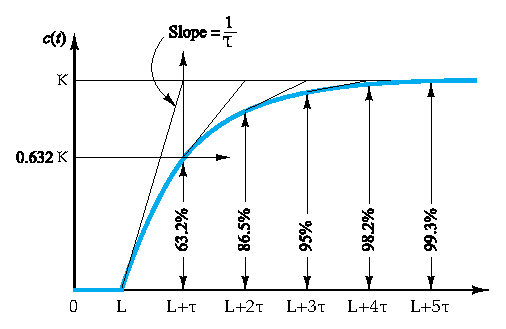
\includegraphics[width=10cm]{images/firstOrder+deadTimeResponse.eps}
 \end{column} 
\end{columns}
\end{frame}

\begin{frame}[<-+>]\frametitle{Sistemas de Segundo Orden - Respuesta Paso}
\vspace*{3mm}
\begin{columns}
 \begin{column}{0.3\textwidth}
  \begin{equation*}
    H(s) = \frac{\omega_n^2}{s^2 + 2 \zeta \omega_n s + \omega_n^2}
  \end{equation*}
  $\omega_n$: Frecuencia natural\\
  $\zeta$: Factor de amortiguamiento\\
  \vspace*{5mm}
  $\zeta < 1$: subamortiguado\\
  $\zeta = 1$: críticamente amortiguado\\
  $\zeta > 1$: sobreamortiguado

 \end{column} 
 \begin{column}{0.7\textwidth}
  \centering
  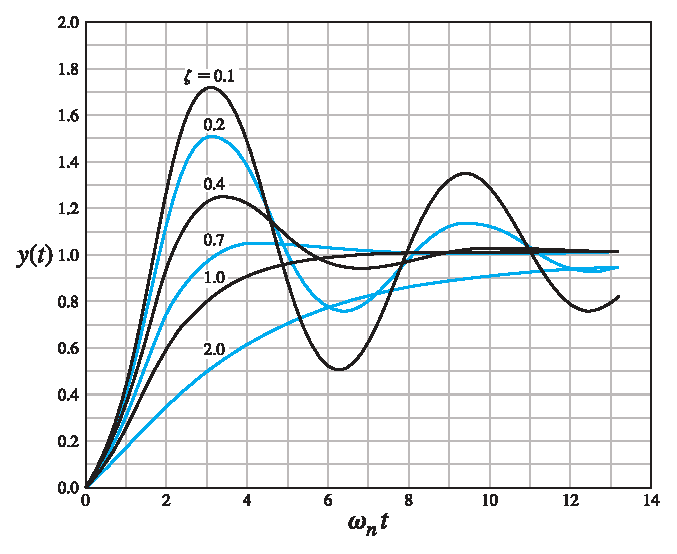
\includegraphics[width=9cm]{images/secondOrderResponse.eps}
 \end{column} 
\end{columns}
\end{frame}

\begin{frame}[<-+>]\frametitle{Respuesta Transitoria}
  La respuesta transitoria del sistema puede describirse en función de dos factores:
  \begin{itemize}
    \item La \textbf{rapidez de la respuesta}, la cual está representada por el \textbf{tiempo de subida} y el \textbf{tiempo pico}.
    \item La \textbf{proximidad de la respuesta al valor final}, representada por el \textbf{sobrepico} y el \textbf{tiempo de establecimiento}.
  \end{itemize}
\end{frame}

\begin{frame}[<-+>]\frametitle{Respuesta Transitoria}
  \begin{itemize}
    \item \textbf{Tiempo de subida} ($T_r$): Tiempo que tarda la respuesta en ir del 10\% al 90\% del valor final.
    \item \textbf{Tiempo pico} ($T_p$): Tiempo en el cual la respuesta alcanza el valor máximo.
    \item \textbf{Sobrepico} ($PO$): Relación en porcentaje entre el valor máximo y el valor final.
    \item \textbf{Tiempo de establecimiento} ($T_s$): Tiempo que tarda la respuesta en mantenerse dentro de un 2\% del valor final.
  \end{itemize}
\end{frame}

\begin{frame}[<-+>]\frametitle{Respuesta Transitoria - Sistemas de Primer Orden}
\vspace*{3mm}
\begin{columns}
 \begin{column}{0.3\textwidth}
 \textbf{Tiempo de subida:}
 \begin{equation*}
   T_r = 2.2 \tau
 \end{equation*}
 \textbf{Tiempo de establecimiento:}
 \begin{equation*}
  T_s = 4 \tau
 \end{equation*}
 \end{column} 
 \begin{column}{0.7\textwidth}
  \centering
  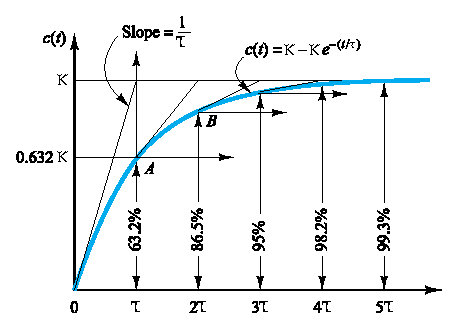
\includegraphics[width=10cm]{images/firstOrderResponse.eps}
 \end{column} 
\end{columns}
\end{frame}

\begin{frame}[<-+>]\frametitle{Respuesta Transitoria - Sistemas de Primer Orden mas Tiempo Muerto}
\vspace*{3mm}
\begin{columns}
 \begin{column}{0.3\textwidth}
 \textbf{Tiempo de subida:}
 \begin{equation*}
   T_r = 2.2 \tau
 \end{equation*}
 \textbf{Tiempo de establecimiento:}
 \begin{equation*}
  T_s = L + 4 \tau
 \end{equation*}
 \end{column} 
 \begin{column}{0.7\textwidth}
  \centering
  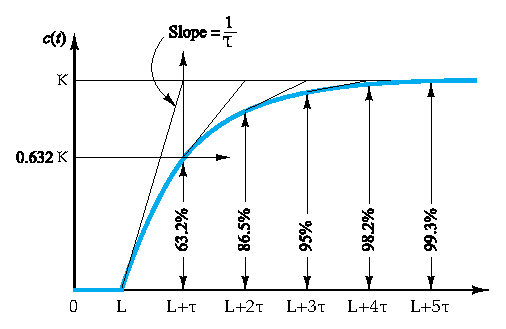
\includegraphics[width=10cm]{images/firstOrder+deadTimeResponse.eps}
 \end{column} 
\end{columns}
\end{frame}

\begin{frame}[<-+>]\frametitle{Respuesta Transitoria - Sistemas de Segundo Orden}
\vspace*{3mm}
\begin{columns}
 \begin{column}{0.3\textwidth}
 \textbf{Tiempo de establecimiento:}
 \begin{equation*}
  T_s = 4 \tau = \frac{4}{\zeta \omega_n}
 \end{equation*}
 \textbf{Tiempo de pico:}
 \begin{equation*}
   T_p = \frac{\pi}{\omega_n \sqrt{1-\zeta^2}}
 \end{equation*}
 \textbf{Sobrepico:}
 \begin{equation*}
   PO = 100 e^{-\zeta \pi/\sqrt{1-\zeta^2}}
 \end{equation*}
 \end{column} 
 \begin{column}{0.7\textwidth}
  \centering
  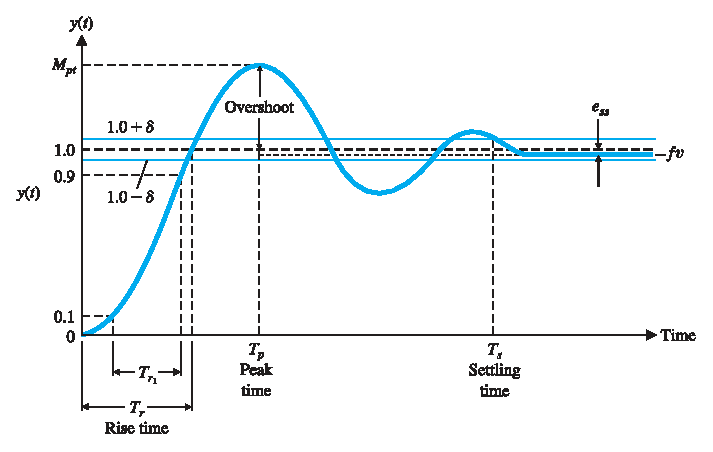
\includegraphics[width=9cm]{images/secondOrderResponseParameters.eps}
 \end{column} 
\end{columns}
\end{frame}

\begin{frame}[<-+>]\frametitle{Respuesta Transitoria - Sistemas de Segundo Orden}
\vspace*{3mm}
\begin{columns}
 \begin{column}{0.3\textwidth}
 \textbf{Tiempo de subida:}
 \begin{equation*}
   T_{r1} = \frac{2.16\zeta + 0.60}{\omega_n}
 \end{equation*}
 Aproximación lineal válida para $0.3 \leq \zeta \leq 0.8$.
 \end{column} 
 \begin{column}{0.7\textwidth}
  \centering
  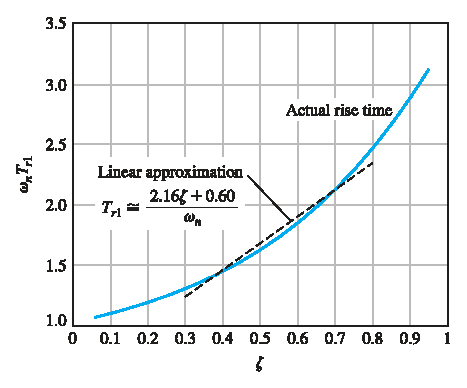
\includegraphics[width=9cm]{images/secondOrderRiseTime.eps}
 \end{column} 
\end{columns}
\end{frame}

\begin{frame}[<-+>]\frametitle{Respuesta Transitoria - Sistemas de Segundo Orden}
\vspace*{3mm}
\centering
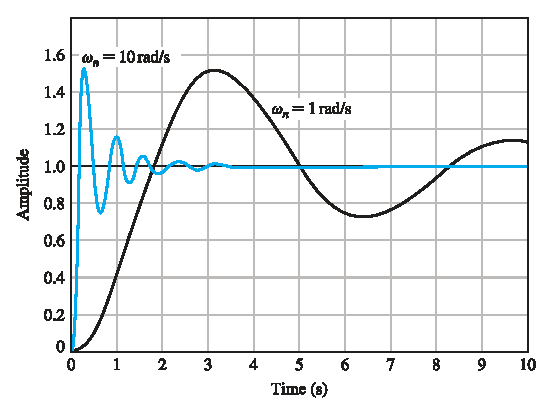
\includegraphics[width=8cm]{images/secondOrderResponseSameZeta.eps}\\
Respuesta paso para $\zeta = 0.2$ con $\omega_n = 1$ y $\omega_n = 10$.
\end{frame}

\begin{frame}[<-+>]\frametitle{Respuesta Transitoria - Sistemas de Segundo Orden}
\vspace*{3mm}
\centering
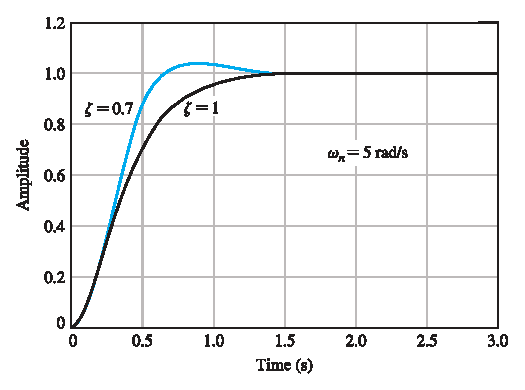
\includegraphics[width=8cm]{images/secondOrderResponseSameOmega.eps}\\
Respuesta paso para $\omega_n = 5$ con $\zeta = 0.7$ y $\zeta = 1$.
\end{frame}

\section{Estabilidad}
\begin{frame}[<-+>]\frametitle{Estabilidad de Sistemas Realimentados}
\begin{itemize}
  \item Estabilidad $\rightarrow$ requerimiento práctico para muchos sistemas.
  \item Sistema inestable $\rightarrow$ puede destruirse o saturarse con cualquier entrada / disturbio.
  \item Dependiendo del tipo de respuesta analizada (estado cero / entrada cero), se consideran dos tipos de estabilidad:
  \begin{itemize}
    \item Estabilidad externa.
    \item Estabilidad interna.
  \end{itemize}
\end{itemize}
\end{frame}

\begin{frame}[<-+>]\frametitle{Estabilidad Externa}
  \begin{itemize}
    \item Señal acotada: no crece indefinidamente. Existe una constante $u_m$ tal que $\norm{u(t)} \leq u_m \leq \infty$.
    \item \textbf{Estabilidad BIBO} (bounded input - bounded output): toda entrada acotada produce una salida acotada.
    \item Estabilidad BIBO $\rightarrow$ se define para respuesta a estado-cero (sistema inicialmente relajado).
  \end{itemize}
  \begin{theorem}
    Un sistema con función de transferencia racional propia $G(s)$ es BIBO estable si y sólo si todos los polos de $G(s)$ tienen parte real negativa, o se encuentran en el lado izquierdo del semiplano complejo, sin incluir el eje imaginario.
  \end{theorem}
\end{frame}

\begin{frame}[<-+>]\frametitle{Estabilidad Interna}
\centering
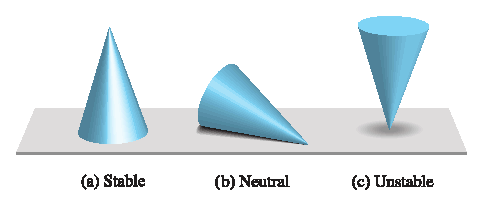
\includegraphics[width=6cm]{images/internalStability.eps}
\begin{itemize}
  \item Se estudia para el caso de respuesta a entrada cero: $\dot{x}(t) = \mathbf{A}x(t)$
  \item Se presentan dos criterios de estabilidad:
  \begin{itemize}
    \item Estable en el sentido de Lyapunov: toda condición inicial limitada genera una respuesta limitada del estado.
    \item Asintóticamente estable: toda condición inicial limitada genera una respuesta del estado limitada que tiende a cero cuando el tiempo tiende a infinito.
  \end{itemize}
\end{itemize}
\end{frame}

\begin{frame}[<-+>]\frametitle{Estabilidad Interna}
\begin{theorem}
\begin{itemize}
  \item El sistema es asintóticamente estable si y sólo si todos los valores propio de $\mathbf{A}$ tienen parte real negativa.
  \item El sistema es marginalmente estable si y sólo si todos los valores propios de $\mathbf{A}$ tienen parte real cero o negativa, y aquellos con parte real cero son raices simples del polinomio característico de $\mathbf{A}$.
\end{itemize}
\end{theorem}
\end{frame}

\begin{frame}[<-+>]\frametitle{Estabilidad}
   En general, los polos de $G(s)$ son un subconjunto de los valores propios de $\mathbf{A}$.
   \begin{itemize}
     \item Si el sistema es asintóticamente estable, entonces el sistema es BIBO estable.
     \item Si el sistema es BIBO estable, el sistema no necesariamente será asintóticamente estable.
     \item Si el sistema no es asintóticamente estable, no se puede hacer afirmación alguna sobre su estabilidad BIBO.
   \end{itemize}
\end{frame}

\begin{frame}[c]\frametitle{Taller}
\begin{enumerate}
  \item Para el sistema mostrado en la figura, considere como entrada la fuerza aplicada sobre la masa de la izquierda, y la salida como la distancia entre las dos masas. Obtenga las ecuaciones diferenciales que describen el sistema, la representación en el espacio de estados y la función de transferencia.
  \seti
\end{enumerate}
\begin{center}
  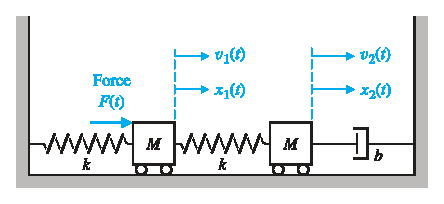
\includegraphics[width=8cm]{images/twoMassSystem.eps}
\end{center}
\end{frame}

\begin{frame}[c]\frametitle{Taller}
\begin{enumerate}
  \conti
  \item El control de inyecciones de insulina puede permitir mejorar la calidad de vida de pacientes diabéticos. La inyección automática de insulina usando una bomba y un sensor que mide los niveles de azucar en la sangre puede ser un tratamiento efectivo. La figura muestra el sistema de control correspondiente a éste proceso. Calcule un valor apropiado para $K$ tal que $PO = 7\%$. Calcule $T_s$ y $T_p$.
  \seti
\end{enumerate}
\begin{center}
  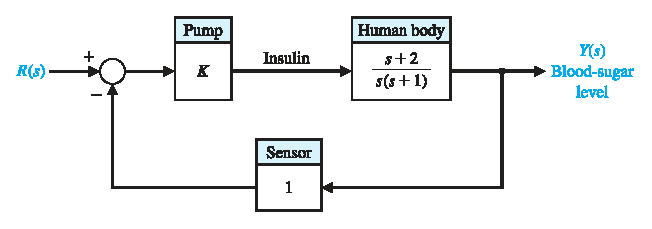
\includegraphics[width=10cm]{images/insulin.eps}
\end{center}
\end{frame}

\begin{frame}[c]\frametitle{Taller}
\begin{enumerate}
  \conti
  \item Para el sistema mostrado en la figura, determine si el sistema es:
  \begin{itemize}
    \item BIBO estable.
    \item Estable en el sentido de Lyapunov.
  \end{itemize}
  \seti
\end{enumerate}
  \begin{center}
    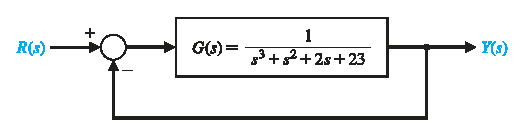
\includegraphics[width=10cm]{images/stability.eps}
  \end{center}
\end{frame}

\begin{frame}[c]\frametitle{Taller}
\begin{enumerate}
  \conti
  \item El sistema mostrado en la figura representa un proceso que controlador por un controlador proporcional-derivativo (PD). Determine el rango de $K_P$ y $K_D$ para garantizar BIBO-estabilidad del sistema en lazo cerrado.
\end{enumerate}
  \begin{center}
    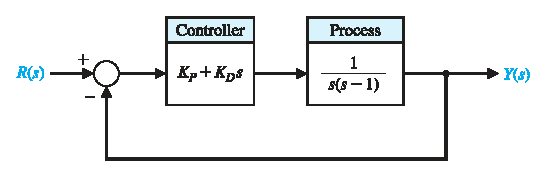
\includegraphics[width=10cm]{images/stability_PD.eps}
  \end{center}
\end{frame}

% \begin{frame}[c]\frametitle{Objetivos del Curso}
% \begin{itemize}
%   \item Posicionar el control de sistemas en el contexto de automática.
%   \item Definir y analizar especificaciones de desempeño de un sistema de control lineal e invariante.
%   \item Modificar la respuesta dinámica de sistemas mediante sistemas de control.
%   \item Seleccionar un controlador y sus parámetros óptimos para un problema dado.
%   \item Reconocer y plantear alternativas de solución a los problemas básicos de control.
% \end{itemize}
% \end{frame}

% \begin{frame}[<+->]\frametitle{Estrategias Pedagógicas del Curso}
% \begin{itemize}
%   \item Asignación de lecturas para estudio individual anterior y posterior a la clase.
%   \item Exposiciones teóricas por parte del profesor (sesiones teóricas).
%   \item Desarrollo de proyectos de aplicación (sesiones prácticas).
%   \item Uso de herramientas de simulación y diseño de controladores.
% \end{itemize}
% \end{frame}

% \begin{frame}[c]\frametitle{Actividades de Evaluación del Curso}
% \centering
% \begin{tabular}{c|c|c}
%   \textbf{Componente}     & \textbf{Fecha}    & \textbf{Valor}\\
%   \hline
%   Examen parcial & Semana 9 & 30\% \\
%   Examen final & Semana 17 & 30\% \\
%   Talleres & Semana 16 & 20\% \\
%   Tareas & Permanente & 20\%
% \end{tabular}
% \end{frame}

% \begin{frame}[<+->]\frametitle{Contenidos Generales del Curso}
% \textbf{Capítulo 1: Introducción al Control:}
% \begin{itemize}
%   \item Semana 1: 
%   \begin{itemize}
%     \item Introducción a la automatización: estructura jerárquica, dominios de control.
%     \item Definiciones y términos asociados a los sistemas de control.
%     \item Estructura de un sistema de control de lazo cerrado.
%     \item Definición de bloques y variables
%   \end{itemize}
%   \item Semana 2:
%   \begin{itemize}
%     \item Especificaciones de desempeño.
%     \item Modelo en espacio de estados y función de transferencia.
%     \item Respuesta en el tiempo (FOL, FOLPDT, SO, resumen).
%     \item Error en estado estacionario.
%     \item Estabilidad.
%   \end{itemize}
%   \seti
% \end{itemize}
% \end{frame}

% \begin{frame}[<+->]\frametitle{Contenidos Generales del Curso (cont)}
% \textbf{Capítulo 2: Sintonización de Controladores:}
% \begin{itemize}
%   \conti
%   \item Semana 3:
%   \begin{enumerate}
%     \item Acciones de control y controladores.
%     \begin{itemize}
%       \item Controladores de dos posiciones (ON-OFF).
%       \item Controladores de tres términos: P, PI, PID.
%     \end{itemize}
%   \end{enumerate}
%   \item Semana 4:
%   \begin{enumerate}
%     \item Criterios clásicos de sintonización (no óptimos):
%     \begin{itemize}
%       \item Modelos aproximados FOPDT.
%       \item Métodos de Ziegler-Nichols, Cohen-Coon.
%     \end{itemize}
%     \item Criterios de sintonización óptima:
%     \begin{itemize}
%       \item Índices de desempeño.
%       \item Sintonía por criterios IAE, ITAE, ISE.
%     \end{itemize}
%   \end{enumerate}
%   \item Semana 5: Sesión de Matlab:
%   \begin{itemize}
%     \item Síntesis de controladores: método matemático por igualación de funciones características.
%   \end{itemize}
%   \seti
% \end{itemize}
% \end{frame}

% \begin{frame}[<+->]\frametitle{Contenidos Generales del Curso (cont)}
% \textbf{Capítulo 3: Diseño de compensadores por lugar geométrico de las raíces (LGR) y respuesta en frecuencia:}
% \begin{itemize}
%   \conti
%   \item Semana 6:
%   \begin{enumerate}
%     \item Diseño de compensadores por LGR.
%     \item Aproximación de polos dominantes.
%   \end{enumerate}
%   \item Semana 7:
%   \begin{enumerate}
%     \item Diseño de compensador en adelanto.
%     \item Diseño de compensador en atraso.
%     \item Diseño de compensador en adelanto-atraso.
%   \end{enumerate}
%   \seti
% \end{itemize}
% \end{frame}

% \begin{frame}[<+->]\frametitle{Contenidos Generales del Curso (cont)}
% \begin{itemize}
%   \conti
%   \item Semana 8: Diseño en el dominio de la frecuencia:
%   \begin{itemize}
%     \item Respuesta en frecuencia: diagramas de Bode, márgenes de fase y ganancia.
%     \item Compensador en adelanto.
%   \end{itemize}
%   \item Semana 9: \textbf{Examen parcial.}
%   \item Semana 10: Sesión de Matlab
%   \begin{enumerate}
%    \item Diseño de compensador en atraso.
%    \item Diseño de compensador en adelanto-atraso.
%   \end{enumerate}
%   \item Semana 11: Sesión de Matlab
%   \seti
% \end{itemize}
% \end{frame}

% \begin{frame}[<+->]\frametitle{Contenidos Generales del Curso (cont)}
% \textbf{Capítulo 4: Sistemas de control en tiempo discreto:}
% \begin{itemize}
%   \conti
%   \item Semana 12: Sesión de Matlab
%   \item Semana 13: Elementos de un sistema de control digital
%   \begin{enumerate}
%     \item Diagrama de bloques.
%     \item Sistemas de datos muestreados.
%     \item Funciones de transferencia.
%     \item Correspondencia entre los planos $s$ y $z$.
%     \item Presentación de proyecto.
%   \end{enumerate}
%   \seti
% \end{itemize}
% \end{frame}

% \begin{frame}[<+->]\frametitle{Contenidos Generales del Curso (cont)}
% \begin{itemize}
%   \conti
%   \item Semana 14: Controladores discretos
%   \begin{itemize}
%     \item Médotos de discretización de controladores.
%     \begin{itemize}
%       \item PID discreto.
%       \item Transformación backward, forward, bilineal.
%     \end{itemize}
%     \item Diseño de controladores digitales
%     \begin{itemize}
%       \item Diseño por LGR en el plano $z$
%     \end{itemize}
%   \end{itemize}
%   \item Semana 15, 16: Sesión de Matlab - Implementación de Algoritmos.
%   \item Semana 17: Entrega de proyecto.
%   \item Semana 18: \textbf{Examen final.}
%   \seti
% \end{itemize}
% \end{frame}

% \begin{frame}[c]\frametitle{Bibliografía del Curso}
% \small
% \textbf{Texto guía:}
% \begin{itemize}
%   \item Dorf, R. C., Bishop, (2011). Sistemas de control moderno. Pearson Prentice Hall.
% \end{itemize}
% \textbf{Otras referencias:}
% \begin{itemize}
%   \item Franklin, G. F., Powell, J. D., \& Workman, M. L. (2006). Digital control of dynamic systems. Menlo Park: Addison-wesley.
%   \item Golnaraghi, F., \& Kuo, B. C. (2010). Automatic control systems. Wiley.
%   \item CHEN Chi-Tsong. ANALOG AND DIGITAL CONTROL SYSTEM DESIGN: Transfer-Function,State-Space, and Algebraic Methods. Philadelphia: Saunders College, 1993.
%   \item SMITH Carlos A. and CORRIPIO Armando. PRINCIPLES AND PRACTICE OF AUTOMATIC PROCESS CONTROL - 2nd. Edition. New York: John Wiley and Sons. 1997.
% \end{itemize}
% \end{frame}

% \begin{frame}[<+->][c]\frametitle{Declaración de los Reglamentos}
% \footnotesize
% \begin{itemize}
%   \item 113. Constituyen faltas graves:
%   \begin{itemize}
%     \footnotesize
%     \item d. El fraude en actividades, trabajos y evaluaciones académicos y la posesión o utilización de material no autorizado en los mismos.”
%   \end{itemize}
%   \item “118. Adicional a la sanción disciplinaria, el fraude en actividades, trabajos y evaluaciones académicos se sancionará académicamente con la pérdida de la asignatura, la cual será calificada con nota definitiva de cero punto cero (0.0)”
%   \item “120. Además de la sanción disciplinaria, el plagio o la suplantación en una evaluación académica, en exámenes preparatorios, en trabajo de grado y tesis, se sancionarán académicamente con la pérdida de la asignatura la cual será calificada con nota definitiva de cero punto cero (0.0).”
%   \item “67. Evaluación supletoria es aquella que remplaza otra evaluación académica que el estudiante no pudo presentar oportunamente, por razones debidamente justificadas por escrito ante el Director del Programa. Dicha justificación deberá presentarse en un plazo no superior a los cinco días hábiles siguientes a la fecha de la evaluación no presentada.”
% \end{itemize}
% \end{frame}

% \begin{frame}[c]\frametitle{Comunicación durante el curso}
% \begin{itemize}
%   \item Discord: \url{https://discordapp.com/download}
%   \item Enlace de invitación al servidor privado: \url{https://discord.gg/R5XnvFM}
%   \item Contenidos del curso.
%   \item Trabajos propuestos.
%   \item Discusiones y preguntas.
% \end{itemize}
% \end{frame}

% \section{Fundamentos de Sistemas de Control}

% \begin{frame}[<+->][c]\frametitle{Control de Sistemas - Contexto General}
%   \textbf{Automática:}
%   \begin{itemize}
%     \item Ciencia que estudia los métodos y procedimientos que permiten la sustitución del operador humano por uno artificial, en una tarea previamente programada.
%   \end{itemize}
%   \textbf{Automatización:}
%   \begin{itemize}
%     \item Es la realización de tareas y funciones mediante máquinas de funcionamiento autónomo, sin la intervención directa del hombre.
%   \end{itemize}
% \end{frame}

% \begin{frame}[c]\frametitle{Control de Sistemas - Importancia}
% \textbf{Por qué es importante el control?}
% \begin{itemize}
%   \item En robótica: \href{https://www.youtube.com/watch?v=wlkCQXHEgjA}{(video)} \href{https://www.youtube.com/watch?v=_sBBaNYex3E}{(video)}
%   \item En la industria automotriz: \href{https://www.youtube.com/watch?v=rbki4HR41-4}{(video)}
%   \item En vehículos autónomos: \href{https://www.youtube.com/watch?v=tlThdr3O5Qo}{(video)}
%   \item En la industria aeronáutica: \href{https://www.youtube.com/watch?v=GrP3jHuLQ9o}{(video)}
% \end{itemize}
% \end{frame}

% \begin{frame}[<+->][c]\frametitle{Control de Sistemas - Introducción}
% \begin{itemize}
%   \item Ingenieros $\rightarrow$ crean productos para ayudar a las personas.
%   \item Entender, modelar y controlar materiales y fuerzas de la naturaleza.
%   \item Ingeniería de sistemas de control:
%   \begin{itemize}
%     \item Área de la ingeniería que busca entender, modelar y controlar segmentos del ambiente, llamados \textbf{sistemas}.
%     \item Basada en los principios de teoría de retroalimentación, análisis de sistemas lineales.
%     \item Fuertes fundamentos matemáticos y gran aplicabilidad en diversas áreas.
%   \end{itemize}
% \end{itemize}
% \end{frame}

% \begin{frame}[<+->][c]\frametitle{¿Qué es un sistema?}
% \begin{center}
%   \includegraphics[width=12cm]{images/planeSystem.png}
% \end{center}  
% \end{frame}

% \begin{frame}[<+->][c]\frametitle{¿Qué es un sistema?}
% \begin{center}
%   \includegraphics[width=12cm]{images/biologySistem.png}
% \end{center}  
% \end{frame}

% \begin{frame}[<+->][c]\frametitle{¿Qué es un sistema?}
% \begin{center}
%   \includegraphics[width=12cm]{images/socialNetwork.png}
% \end{center}  
% \end{frame}

% \begin{frame}[<+->][c]\frametitle{Sistema}
% \begin{itemize}
%   \item Interconexión de componentes, dispositivos o subsistemas.
%   \item Proceso que toma unas entradas y las transforma en salidas.
%   \begin{center}
%     \includegraphics[width=6cm]{images/sistema.png}
%   \end{center}
%   \item Relación entrada - salida: representa la relación causa - efecto del proceso.
%   \item Existe una frontera que separa los componentes internos del mundo externo.
%   \item Enfoque sistemático para analizar el comportamiento: modelos matemáticos.
% \end{itemize} 
% \end{frame}

% \begin{frame}[<+->][c]\frametitle{Sistema de Control}
% \begin{itemize}
%   \item Interconexión de componentes que forman una configuración que provee una respuesta deseada.
%   \item Sistema de control de lazo abierto: Usa un \textbf{controlador} y un \textbf{actuador} para obtener la respuesta del proceso deseada.
%   \begin{center}
%     \includegraphics[width=8cm]{images/openloopcontrol.png}
%   \end{center}  
%   \item Sistema de control de lazo cerrado: Utiliza una medida adicional de la salida para compararla con la respuesta deseada.
%   \begin{center}
%     \includegraphics[width=10cm]{images/closedloopcontrol.png}
%   \end{center}  
% \end{itemize}
% \end{frame}

% \begin{frame}[<+->][c]\frametitle{Sistema de Control}
%   \vspace*{-0.2cm}
%   \begin{center}
%     \includegraphics[width=10cm]{images/closedloopcontrol2.png}
%   \end{center}
%   \vspace*{-0.7cm}
%   \begin{itemize}
%     \item Referencia (set-point): valor deseado de la variable controlada.
%     \item Variable controlada: cantidad o condición que se mide y controla. Normalmente es la salida del sistema.
%     \item Variable manipulada: cantidad o condición que el controlador modifica para afectar el valor de la variable controlada.
%     \item Perturbación: señal externa que ocasiona que la variable de control se desvíe del punto de control.
%   \end{itemize}
% \end{frame}

% \begin{frame}[<+->][c]\frametitle{Sistema de Control}
%   \vspace*{-0.2cm}
%   \begin{center}
%     \includegraphics[width=10cm]{images/closedloopcontrol2.png}
%   \end{center}
%   \vspace*{-0.7cm}
%   \begin{itemize}
%     \item Ruido de medida: señal externa que contamina la medición hecha con el sensor sobre la variable controlada.
%     \item Error: Diferencia entre la referencia y la medición obtenida mediante el sensor.
%   \end{itemize}
% \end{frame}

% \begin{frame}[c]\frametitle{Sistemas de Control - Ejemplos: Vehículos autónomos}
%   \begin{center}
%     \includegraphics[width=8cm]{images/controlsystem_example1.png}
%   \end{center}
% \end{frame}

% \begin{frame}[c]\frametitle{Sistemas de Control - Ejemplos: Operador humano en el lazo de control}
%   \begin{center}
%     \includegraphics[width=9cm]{images/controlsystem_example2.png}
%   \end{center}
% \end{frame}

% \begin{frame}[c]\frametitle{Sistemas de Control - Ejemplos: Ingresos en una nación}
%   \begin{center}
%     \includegraphics[width=10cm]{images/controlsystem_example3.png}
%   \end{center}
% \end{frame}

% \begin{frame}[c]\frametitle{Diseño de Sistemas de Control}
%   \begin{columns}
%     \begin{column}{0.4\textwidth}
%        \textbf{Objetivo:} Obtener la configuración, especificaciones e identificación de los parámetros clave del sistema propuesto para satisfacer los requerimientos.
%     \end{column}
%     \begin{column}{0.6\textwidth}
%       \begin{center}
%         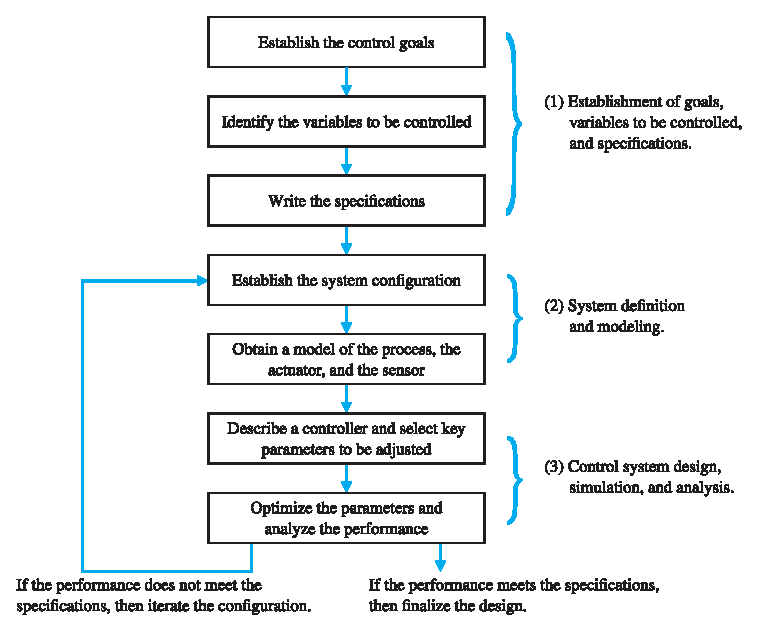
\includegraphics[width=8cm]{images/controlsystemdesign.eps}
%       \end{center}
%     \end{column}
%   \end{columns}
% \end{frame}

% \begin{frame}[c]\frametitle{Taller - Sistemas de Control}
% \begin{enumerate}
%   \item Describa sensores típicos que puedan usarse para medir las siguientes variables:
%   \begin{itemize}
%     \item Posición lineal
%     \item Posición rotacional
%     \item Temperatura
%     \item Presión
%     \item Fuerza
%     \item Flujo de líquido
%     \item Campo magnético terrestre
%   \end{itemize}
%   \item Describa actuadores típicos que puedan convertir las siguientes variables:
%   \begin{itemize}
%     \item Energía eléctrica en energía mecánica
%     \item Deformación mecánica en energía eléctrica
%     \item Energía química en energía cinética
%     \item Calor en energía eléctrica
%   \end{itemize}
%   \seti
% \end{enumerate}
% \end{frame}

% \begin{frame}[c]\frametitle{Taller - Sistemas de Control (cont)}
% \begin{enumerate}
%   \conti
%   \item Una cámara con foco automático ajusta la distancia entre el lente y el sensor usando un rayo infrarojo para determinar la distancia al objetivo. Realice un bosquejo del diagrama de bloques de éste sistema de control especificando los diferentes componentes y señales. Explique brevemente su operación.
%   \seti
% \end{enumerate}
% \end{frame}

% \begin{frame}[c]\frametitle{Taller - Sistemas de Control (cont)}
% \begin{columns}
%   \begin{column}{0.5\textwidth}
%     \begin{enumerate}
%       \conti
%       \item Considere el péndulo invertido mostrado en la figura. El objetivo es mantener el péndulo en la posición vertical ($\theta = 0$) en la presencia de disturbios. Realice el bosquejo del diagrama de bloques del sistema de control. Identifique el proceso, sensor, actuador y controlador.
%     \end{enumerate}
%   \end{column} 
%   \begin{column}{0.5\textwidth}
%    \centering
%    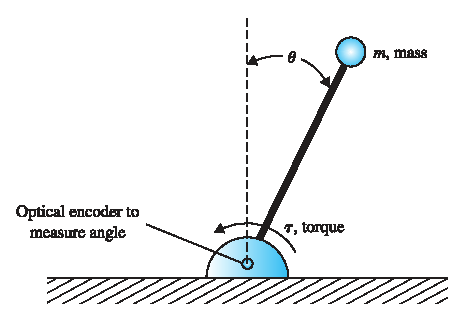
\includegraphics[width=6cm]{images/invertedpendulum.eps}
%   \end{column} 
% \end{columns}
% \end{frame}

\end{document}